\documentclass[11pt,a4paper]{article}
\usepackage[latin1]{inputenc}
\usepackage{amsmath}
\usepackage{graphicx}
\usepackage{amsfonts}
\usepackage{amssymb}
\title{On analyzing large graphs}
\author{}
\begin{document}
\maketitle


This article first introduces JMaxGraph, a Java library for the analysis of large graph topologies.

By large we mean so large that standard tools for graph processing cannot be used.

This article enumerates the obstacles we faced, and it exposes the solutions we had
to find for each of them in order to reach our goal.


As an example, the use case we present in this paper uses the graph of Twitter users.
The data connecting users in Twitter was collected by the DIANA research group (Inria) in 2011. It comes as a single 215GB text file, in the ADJ format. It stores 
398,846,191 vertices and 23,137,510,395 arcs.




\section{Other graph analysis tools}

Sage, NetworkIt and NetworkX are written in Python. They are highly flexible libraries which are easily usable through the Python interpreter. They compensate the inherent slowness of interpreted Python by offering a facilities and bridges to algorithms written in C. Unfortunately the overhead of frequently switching context between Python and C result in poor performance.

JGraphT and Jung are Java libraries. Their offer a similar Object-oriented model. They both are written in Java, using idiomatic programming paradigm, therefore they both suffer from  the heavy memory model of the JVM. Indeed in the Hotspot JVM, object overhead is 8 bytes and every object occupies a number of bytes that is a multiple of 8. If the number of bytes required by an object for its header and fields is not a multiple 8, then you round up to the next multiple of 8. As a consequence, an instance of a Vertex class with one single int field to store the ID of the vertex  occupies 16 bytes in memory, where it should has only 4 bytes. Each reference to this instance uses 8 more bytes (in a 64bit memory model). Note that if an object is not referenced, it is destroyed by the garbage collector.

The Grph library overcomes this drawback by representing vertices and edges by primitive integers (int values). It accomplishes this by relying on the Fastutil library. 

Hadoop Giraph is a Java distributed graph library build on top of Apache Hadoop. It uses in-memory compression in order to save RAM.
GraphX is a distributed graph library build on top of Spark. It is written in Scale and therefore makes exclusive use of the functional programming paradigm. This feature makes its difficult to non-specialists. GraphX turned out not to scale well because the immutable data model is relies on uses huge amount of memory. Also the results it returns were sometimes wrong.
Both Giraph and GraphX partition the graph across the nodes of computational cluster. The solve the inherent complexity of distributed computing by proposing the BSP programming model. BSP is a vertex-centric message-based programming model which is very adequate to the implementation of simple vertex-centric algorithms. Unfortunately it cannot be used for algorithms that have no natural vertex-centric expression, for which it imposes poor performance because of network congestion due to too numerous messages transiting.
Even vertex-centric algorithm suffer from the distributed nature of the data because the overhead of transiting algorithm local states severely impedes performance.

GraphChi leaves the graph on disk. It proposes an efficient loading mechanism in order to enable on-the-fly processing.

WebGraph is a centralized library written in Java. Its data-structure 
uses compression in order to allow large graphs to fit in RAM. Using this data-structure imposes a compromise between decompression-overhead and compression ratio.

\section{JMaxGraph}

JMaxGraph benefits from our experience in dealing with existing libraries and programming paradigms for graph algorithms.
Its main features are:
\begin{enumerate}
\item it is written in Java for its portability, industrial-class strength and popularity
\item it supports both in-memory (uncompressed) and disk-based (compressed) operations. An algorithm can use both at the same time.
\item its data-structure uses lowest-level abstraction in order to avoid Java overhead when dealing with objects
\item it makes extensive use of multi-threading in order to take full advantage of multi-core computers (in today's clusters, no node have less that 16 cores)
\item it uses a custom file-system based Map/Reduce distributed computation engine. It order to enable large experimentation campaigns, it is able to recover on error thanks to its incremental job system.
\end{enumerate}

In order to allow this, JMaxGraph has a number restriction:

\begin{enumerate}
\item vertices are numbers --- not objects --- leaving to the user the responsibility to provide a bridge to its OO model if any.
The vertex ID space is contiguous, ranging from 0 to N-1, N being the number of vertices in the graph.
\item it does not store edges, nor it stores values for edges
\end{enumerate}


\subsection{In-memory data-structure}

The adj-list are stored in an array. Neighbors of vertex $u$ can in found at the $u^{th}$ cell, referred to as $adj[u]$.
Adj-list are ordered. The $u^{th}$ neighbor of vertex $u$ can be obtained by $adj[u][i]$.

This allows $O(log(n))$ search for a given arc.

JMaxGraph exposes the $int[][]$ to algorithm for the following reason: the graph data can hence be accessed in direct, with no need to do through methods, which woul impose a JMG, passing parameter, thereby manipulation the thread stack. Performance greatly benefits from using this low-level approach.

Java Arrays have another significant advantage: they can be accessed in parallel by threads with no performance loss. Several threads working on distinct areas of an array are then not be slowed done by each other nor they generate inconsistent values.

\section{On-disk storage: the JMG data format}

The Twitter graph initially came as an ADJ file. The ADJ file format defines that the first line of the file is the number of vertices. Each following line then consists of:
\begin{enumerate}
\item the ID of the vertex;
\item the number of neighbors;
\item the ID for each neighbor.
\end{enumerate}
Numbers are separated by a space.


Using 16MB buffer.
The read throughput of the cluster is 600MB/s. Transferring the entire file to RAM takes 7min.

Using Java standard buffering I/O and number parsing, loading the entire graph takes min. The read throughput then MB/s.

1
2
4
8		4.5=>2.5
16
32

We profiled the execution and we discovered that both  the  basic I/O primitives for reading data from the file and the number parsing methods dramatically slowed down the process. By analyzing the source code of the Java standard library, we found out that the responsible is the excessive number of method calls. These methods had not been in-lined by the just-in-time compiler.

We made a new implementation of buffered reading and number parsing, which speeds up the graph loading process by a factor 30, as illustrated on Figure \ref{fig-a}. Thereby reducing the loading time to 7min. We can see that the graph loading speed is very close to the speed of pure data transfer to memory, which means that the time spent turning text data to graph data-structure is insignificant. Thus at this point, the bottleneck becomes the disk reads. This motivated the definition of a the JMG file format.


\begin{figure}
\begin{center}
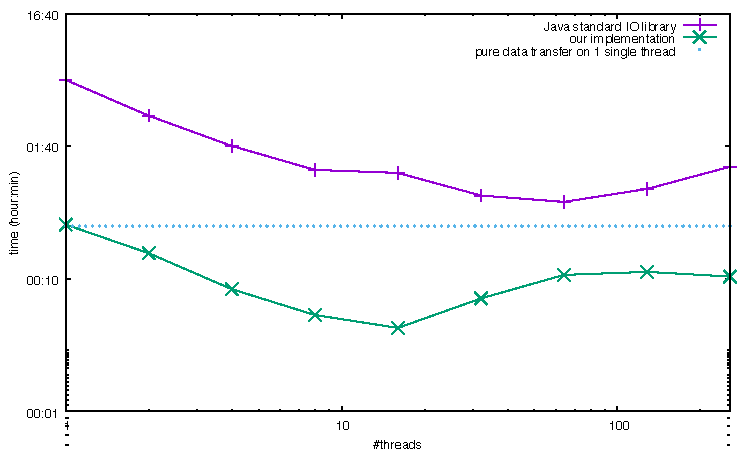
\includegraphics[width=0.8\linewidth]{load.pdf}
\end{center}
\caption{blabla}
\end{figure}

In the JMG format, the graph is described by several files in a directory. Two file types:

The \texttt{properties.txt}  is an ASCII text file. It consists of a sequence of $key=value$ lines. It stores various graph property, such as the number of vertices in the graph.

ARC files store adjacencies. A JMG directory embeds at least one ARC file, which stores either the OUT-adj or the IN-adj. But it may contain the ARC files for both directions.
The IN (resp. OUT) adjacency is expected to be found in a file \texttt{in.arc} (resp. \texttt{out.arc}). Such ARC file comes with its index file, called \texttt{-index.nbs}. An NBS file is a binary fixed-length encoding for integer numbers.
For each vertex $u$, the index file has an entry which gives the position in the adjacency file at which the set of neighbors of $u$ are stored.

In the ARC file, this set of neighbors is encoded at a byte sequence of length:
$$l = index(u+1) - index(u)$$
 Note that if $u$ is the vertex with the highest ID,  they does not exist such thing as $index(u+1))$. The length of the byte sequence describing its neighborhoods is then defined by:
 $$l = size(indexFile) - index(u)$$
Note also that the number neighbors cannot be computed out of this $l$, as every vertex may use words of different length to store their neighborhood.
Then, starting at position $index(u)$, the byte sequence encoding the set of neighbors for vertex $u$ is organized like this:
\begin{enumerate}
\item 8 bytes encode the neighbor with lowest ID
\item 1 byte encodes the number of bytes used to store each other neighbor, let us refer to it as $e$. The number of neighbors is then defined by $1 + \frac{l - 9}{e}$.
\item each following neighbor $v_i$ of $u$ is encoded as the delta $d$ of its ID and the ID of the previous neighbor.
The ID of the $i^{th} (with\ i > 0)$ neighbor is obtained by:
$$v_i = v_{i-1} + d$$.
\end{enumerate}

The JMG file format exhibits the following advantages:
\begin{enumerate}
\item adjacency lists are ordered, which is very profitable to algorithms which can hence resort to dichotomy.
\item the dataset can be accessed randomly. This means that the degree and the adjacency of any given vertex can be retrieved from disk without having to load/parse other vertices.
\item an ARC file is iterable. This means that adj-list contains in an ARC file can be processed on-the-fly when the file is loaded. This mechanism fastens algorithms which process any adj-list one single time and make it possible to execute certain algorithms even though there is not enough RAM to load the entire graph.
\item there is no vertex in adjacency lists that is not in the vertex set.
\item adjacency lists are compressed in such a way that the more an adj-list is long, the fewer bytes will be used to store each individual element.
\item compression/decompression time is insignificant
\end{enumerate}

The Twitter datasets is 3-times smaller when encoded as a JMG datasets rather than stored in an ADJ file.


\section{Graph processing models}

\subsection{Sequential}

Benefits from direct-access to Java arrays

\subsection{Multi-threaded}

Benefits from concurrent nature of Java arrays.


\subsection{Map/Reduce}
one job per file
large number of jobs in order to allow better distribution accros cluster nodes

inherently incremental, meaning that job result are stored in a file as soon as it is computed. No job will be computed twice. Which makes it resilient to failures because when/if the system gets restarted, it will continue computation at the stage it was.
distributed, with no restriction whatsoever on the number of workers 

\section{Algorithms}

\subsection{Counting K2,2 and triangles}

Do we include this?

\subsection{Tarjan}

sequential

optimized

parallel

\subsection{Kernighan-Lin}



\section{Additional features}

\subsection{Progress monitoring}

Algorithms on large datasets often have unknown expected termination date. They will run for a long time, hours days or even months. It is of paramount importance to have information on the running process, in particular an indication of its progress, and a view of its current state (intermediary results).

\end{document}